\chapter{群}
近世代数的基石是群的概念。群是拥有丰富而有趣理论的最简单代数结构之一,几乎所有数学中出现的代数结构都包含群。此外,它们对于我们理解数学物理中的一些基本概念,尤其是与对称性有关的概念,也非常重要。

群的概念起源于埃瓦里斯特-伽罗瓦(Evariste Galois,1811-1832 年)和尼尔斯-亨里克-阿贝尔(Niels Henrik Abel,1802-1829 年)关于用根式解代数方程的研究。后一位数学家以满足交换律的一类特殊群组(称为阿贝尔群组)的名称而闻名。近代,埃米-诺特(Emmy Noether,1888- 1935 年)发现,由作用原理产生的方程组的每一组对称性都会产生守恒量。例如,能量、动量和角动量分别来自时间平移、空间平移和旋转的对称性。在基本粒子物理学中,还有更多的守恒定律与诸如 SU(3) 这样的奇异基团有关,对它们的理解已经促成了新粒子的发现。本章将介绍群论的基本思想,并举例说明它们是如何在物理环境中出现的。
\section{群论的元素}\label{sec:2.1}
集合 $G$上任意一对 $g,h\in G$,都存在 $gh\in G$称为其\textbf{乘积}(product),满足
\begin{enumerate}
    \item[(Gp1)]\label{gp:1}
    \textbf{结合律}(associative law): 对全体 $g,h,k\in G$有$g(hk)=(gh)k$  
    \item[(Gp2)] \label{gp:2}
    存在\textbf{恒等元}(identity element): $e\in G$,使得对全体\(g\in G\)
    \[eg=ge=g\]
    \item[(Gp3)] \label{gp:3}
    每个群元 $g\in G$有\textbf{逆}(inverse) $g^{-1}\in G$ 使得\[g^{-1}g=gg^{-1}=e\] 
\end{enumerate}
这样的集合称为\textbf{群}(group)

对任意两个元素都存在乘积,且乘积在群内,这个性质称为\textbf{封闭性}(closure property)

类似的,可证明每个$g\in G$ 都有唯一逆 $g^{-1}$且 $(gh)^{-1}=h^{-1}g^{-1}$ 
\\
如果群元可交换,即\[gh=hg\]总成立,则称群是\textbf{阿贝尔的}(abelian),如果群乘法写成加法的形式,那我们默认其是阿贝尔的, $g$ 的逆是$-g$ 

集合 $H\subseteq G$满足:
\begin{enumerate}
    \item[(a)] $h,k\in H\Rightarrow hk\in H$ 
    \item[(b)] $e\in H$ 
    \item[(c)] $h\in H,h^{-1}\in H$ 
\end{enumerate} 
$H$称为 $G$的子群,无需结合律(Gp1),因为结合律自动继承下来了 
\begin{eg}
    以加法为组成法则的整数 $\mathbb{Z}$ 组成一个群,称为整数加法群。严格地说,这个群应该写成 $(\mathbb{Z},+)$,但 "加法 "一词隐含了组成法则。其特征元素是整数 0,任何整数 n 的逆元是-n。偶数整数 $\{0, \pm 2, \pm 4,...\} $ 构成了整数加法群的一个子群。
\end{eg} 
\begin{eg}
    全体实数和加法形成一个群,称为实数加法群(additive group of reals). $e=0$,$x$的逆是 $-x$ ,整数加法群和有理数加法群显然都是 $\mathbb{R}$的子群 。有理数 $\mathbb{Q}$ 关于加法是封闭的,也构成可加实数 $\mathbb{R}$的一个子群,因为数 0 是有理数,如果 $p /q$ 是有理数,那么 $-p /q$ 也是有理数。
\end{eg}
\begin{eg}
    非零实数$\dot{\mathbb{R}}=\mathbb{R}-\{0\}$形成一个群,称作实数乘法群(multiplication group of reals),群乘法是普通乘法,恒等元$e=1$。$x$ 的逆是 $x^{-1}=1 /x$。0 除外,因为它没有倒数。
    类似的,$\mathbb{\dot{Q}}$也是$\mathbb{\dot{R}}$的子群
    $\mathbb{C}$上同样有加法群,$\mathbb{\dot{C}}$上同样有乘法群
\end{eg}
\begin{exercise}
    证明非零有理数 $\mathbb{Q}$ 构成了 $\mathbb{R}$ 的乘法子群。
\end{exercise}
\begin{exercise}
    证明复数 $\mathbb{C}$ 构成一个关于加法的群,并且 $\mathbb{C}=\mathbb{C}-\{0\}$ 是一个关于复数乘法的群。
\end{exercise}
\begin{exercise}
    下面哪些集合构成加法群:(i) 有理数,(ii) 无理数,(iii) 模为 1 的复数?就乘法而言,它们哪个是一个群?
\end{exercise}

由有限个元素组成的群 $G$ 称为有限群。$G$中元素的个数称为其阶,用$|G|$表示。
\begin{eg}
    让 $k$ 是任意自然数,$\mathbb{Z}_k=\{[0],[1],\ldots,[k-1]\}$ 是例 1.3 中定义的模为 $k$ 的整数,模为 $k$ 的加法为合成律

$$
[a]+[b]=[a+b] .
$$
$\mathbb{Z}_k$ 被称为模 $k$ 的加法群。它是一个有限的群,其阶数为 $k$,写作 $\left|\mathbb{Z}_k\right|=k$。将 $\mathbb{Z}_k$ 中的元素写成 $0,1, \ldots, k-1$ 无歧义,而 $[a+b]$ 通常用 $a+b \bmod k$ 来表示。
\end{eg}
\begin{exercise}
    证明模 $k$ 加法的定义不受余数类 $[a]$ 和 $[b]$ 的选择影响。
\end{exercise}
\begin{eg}
 如果一个群 $G$ 有一个元素 $a$,使得它的幂 $\left\{a, a^2, a^3, \ldots\right\}$ 遍历其所有元素,则称 $G$ 为循环群,而 $a$ 称为群的生成元。如果 $G$ 是一个有限的循环群,$a$ 是一个生成元,那么存在一个正整数 $m$,使得 $a^m=e$。如果 $m$ 是最小的这样的整数,那么对于任意 $g \in G$,都可以唯一地写成 $g=a^i$,其中 $1 \leq i \leq m$,因为如果 $g=a^i=a^j$,且 $1 \leq i<j \leq m$,则有矛盾 $a^{j-i}=e$,而 $1 \leq(j-i)<m$。在这种情况下,群被表示为 $C_m$,其阶数为 $\left|C_m\right|=m$。模 $k$ 的加法群是一个阶数为 $k$ 的循环群,但在这种情况下,$a^n$ 的表示方式被替换为
$$
n a=\underbrace{a+a+\cdots+a}_{n} \bmod k .
$$ 
\end{eg}
\begin{eg}
    设 $p>2$ 为任意质数。非零模 $p$ 的整数形成一个阶数为 $p-1$ 的群,其乘法模 $p$ 为

$$
[a][b]=[ab]\equiv ab\mod p,
$$
表示为 $G_p$。单位元显然是余数类 $[1]$,但要证明存在逆元,需要用到数论中的以下结果:如果p和q是相对素数,那么就存在整数k和m使得$k p+m q=1$。由于p是一个素数,如果$[q] \neq[0]$,那么q与p是相对素的,并且对于某些k和m:
$$
\begin{pmatrix}
[m][q]=[1]-[k][p]=[1] .
\end{pmatrix}
$$
因此$[q]$有逆元$[q]^{-1}=[m]$。
\end{eg} 
对于小规模的有限群,组合定律可以以乘法表的形式显示,其中$(i, j)$项指定第i个元素和第j个元素的乘积。例如,这是$G_7$的乘法表:

\begin{tabular}{l|llllll}
$G_7$ & 1 & 2 & 3 & 4 & 5 & 6 \\
\hline 1 & 1 & 2 & 3 & 4 & 5 & 6 \\
2 & 2 & 4 & 6 & 1 & 3 & 5 \\
3 & 3 & 6 & 2 & 5 & 1 & 4 \\
4 & 4 & 1 & 5 & 2 & 6 & 3 \\
5 & 5 & 3 & 1 & 6 & 4 & 2 \\
6 & 6 & 5 & 4 & 3 & 2 & 1
\end{tabular}
\section{变换和排列群}
上述例子中的所有群都是非交换群。非交换群最常见的例子是一类叫做变换群的群。我们回顾第 1.4 节,集合 $X$ 的变换是一个一一对应且到的映射 $g:X\to X$。映射 g 有一个反映射 $g^{-1}:X\to X$,使得 $g^{1}\circ g=g\circ g^{-1}=\mathrm{id}_X$ 让两个变换 g 和 $h$ 的乘积定义为它们的函数组合 $gh=g\circ h$
$$
(gh)(x)=g\circ h(x)=g(h(x)).
$$
$X$的所有变换集合构成一个群,用Transf(X)表示:
\begin{enumerate}
 \item[] 封闭性:如果g和$h$是$X$的变换,那么$gh$ 也是;
 \item[] 结合律{:}\:$f(gh)=(fg)h${;}
 \item[] 恒等元{: }$e= \mathrm{id}_X\in $Transf$( X) ; $
 \item[] 自反性: 如果 $g$ 是 $X$ 上的一个变换,那么 $g^{-1} $也是
\end{enumerate}
封闭性源于这样一个事实:两个变换(可逆映射)的组合会产生另一个可逆映射,因为$(f\circ g)^{-1}=g^{-1}\circ f^{-1}$ 。结合律自动适用于映射的复合,而恒等映射和逆映射是显而易见的。$X$ 的变换群是指 Transf($X$)的任何子群。

如果$X$是一个势为$n$的有限集,那么$X$的变换称为$X$元素的置换。$X=\{1,2,\dots,n\}$的排列群称为阶数为$n$的对称群,记为$S_n$。$S_n$ 的任何子群都称为置换群。$n$元素上的一个置换 $\pi$ 可以用置换符号来表示

\[\pi=\begin{pmatrix}1&2&\dots&n\\a_1&a_2&\dots&a_n\end{pmatrix}\]
其中$a_1=\pi(1),a_2=\pi(2)$, 等等. 同样的置换也可以写成
$$
\pi=\left(\begin{array}{llll}
b_1 & b_2 & \ldots & b_n \\
c_1 & c_2 & \ldots & c_n
\end{array}\right)
$$
其中$b_1, b_2, \ldots,b_n$是按任意顺序排列的数字$1,2, \ldots,n$,$c_1=\pi\left(b_1\right), c_2=$ $\pi\left(b_2\right), \ldots,c_n=\pi\left(b_n\right)$。例如,将四元素集合中的元素 2 和 4 互换的置换 $\pi$ 可以有几种写法、
$$
\pi=\left(\begin{array}{llll}
1 & 2 & 3 & 4 \\
1 & 4 & 3 & 2
\end{array}\right)=\left(\begin{array}{llll}
2 & 3 & 1 & 4 \\
4 & 3 & 1 & 2
\end{array}\right)=\left(\begin{array}{llll}
4 & 1 & 2 & 3 \\
2 & 1 & 4 & 3
\end{array}\right), \text { etc. }
$$
就置换符号而言,如果
$$
\sigma=\left(\begin{array}{cccc}
1 & 2 & \ldots & n \\
a_1 & a_2 & \ldots & a_n
\end{array}\right) \quad \text { and } \pi=\left(\begin{array}{cccc}
a_1 & a_2 & \ldots & a_n \\
b_1 & b_2 & \ldots & b_n
\end{array}\right)
$$
那么它们的乘积就是排列 $\pi \sigma=\pi \circ \sigma$
$$
\pi \sigma=\left(\begin{array}{cccc}
1 & 2 & \ldots & n \\
b_1 & b_2 & \ldots & b_n
\end{array}\right) .
$$
请注意,这种乘积涉及先进行$\sigma$后进行$\pi$的置换,这与它们的书写顺序相反;在这一点上可以有不同的约定。由于乘积是函数复合,因此结合律是有保证的。恒等置换为
$$
\mathrm{id}_n=\left(\begin{array}{llll}
1 & 2 & \ldots & n \\
1 & 2 & \ldots & n
\end{array}\right),
$$
而任何置换的逆定理都由下式给出
$$
\pi^{-1}=\left(\begin{array}{cccc}
1 & 2 & \ldots & n \\
a_1 & a_2 & \ldots & a_n
\end{array}\right)^{-1}=\left(\begin{array}{cccc}
a_1 & a_2 & \ldots & a_n \\
1 & 2 & \ldots & n
\end{array}\right) .
$$

对称群 $S_n$ 是一个阶数为 $n!$ 的有限群,即 $n$ 对象可被置换的方式总数。一般来说,它不是阿贝尔的。例如,在 $S_3$ 中
$$
\left(\begin{array}{lll}
1 & 2 & 3 \\
1 & 3 & 2
\end{array}\right)\left(\begin{array}{lll}
1 & 2 & 3 \\
2 & 1 & 3
\end{array}\right)=\left(\begin{array}{lll}
2 & 1 & 3 \\
3 & 1 & 2
\end{array}\right)\left(\begin{array}{lll}
1 & 2 & 3 \\
2 & 1 & 3
\end{array}\right)=\left(\begin{array}{lll}
1 & 2 & 3 \\
3 & 1 & 2
\end{array}\right)
$$
而
$$
\left(\begin{array}{lll}
1 & 2 & 3 \\
2 & 1 & 3
\end{array}\right)\left(\begin{array}{lll}
1 & 2 & 3 \\
1 & 3 & 2
\end{array}\right)=\left(\begin{array}{lll}
1 & 3 & 2 \\
2 & 3 & 1
\end{array}\right)\left(\begin{array}{lll}
1 & 2 & 3 \\
1 & 3 & 2
\end{array}\right)=\left(\begin{array}{lll}
1 & 2 & 3 \\
2 & 3 & 1
\end{array}\right) .
$$

一种更简洁的排列符号是循环符号。从任意一个要被置换的元素开始,例如 $a_1$。让 $a_2$ 成为对 $a_1$ 应用 $\pi$ 变化的结果,让 $a_3$ 成为对 $a_2$ 应用 $\pi$ 变化的结果,等等。最终,第一个元素 $a_1$ 必须再次出现,比如 $a_{m+1}=a_1$。这就定义了一个循环,写成 $\left(a_1 a_2\ldots a_m\right)$。如果 $m=n$,那么 $\pi$ 就被称为循环排列。如果 $m<n$ 那么取任何一个没有出现在由 $a_1$ 产生的循环中的元素 $b_1$,并在 $\pi$ 下创建一个由 $b_1$ 的连续图像组成的新循环 $\left(b_1 b_2\ldots b_m\right)$。继续下去,直到耗尽所有元素 $1, 2,\dots, n$。置换 \(\pi\)可以写成其循环的 的乘积;例如
$$
\begin{pmatrix}1&2&3&4&5&6&7\\4&5&3&7&2&1&6\end{pmatrix}=(1\:4\:7\:6)(2\:5)(3).
$$

请注意,选择循环中的哪个元素作为第一个成员并不重要,因此,$( 1476) = ( 7614) $和$( 25) = ( 52) $

像 (3) 这样长度为 l 的循环仅仅表示置换 $\pi$ 使元素 3 保持不变。如果我们从符号中完全忽略这样的 l 循环,写成

$$
(1476)(2\:5)(3)=(1\:4\:7\:6)(2\:5).
$$
没有共同元素的循环,书写顺序也无关紧要

$$
(14\:7\:6)(25)=(25)(1\:4\:7\:6).
$$

按照从右到左的顺序,根据循环对每个元素的影响,可以很容易地得到排列组合的乘积。例如
$$
(137)(542)(12)(3467)(146)=(1654)(23)(7)
$$

从$1\to4\to6,6\to1\to2\to5,5\to4,4\to6\to7\to1$,等等。
\begin{exercise}
     用循环符号表示$\{1,2,3\}$上的每个排列组合,并写出$S_{3}$的$6\times6$乘法表。
\end{exercise}
长度为 2 的循环称为交换。每个循环都可以写成交换的乘积
$$
(a_{1}\:a_{2}\:a_{3}\ldots\:a_{n})=(a_{2}\:a_{3})(a_{3}\:a_{4})\ldots(a_{n-1}\:a_{n})(a_{n}\:a_{1}),
$$

由于每个排列 $\pi$ 都是循环的乘积,所以它又是交换的乘积。作为交换积的置换表示一般不是唯一的,但所需的交换次数要么总是奇数,要么总是偶数。为了证明这一点,请考虑同次多项式
\begin{align*}
    f(x_1,x_2,\dots,x_n)&=\prod_{l<j}(x_i-x_j)\\
    &=(x_1-x_2)(x_1-x_3)\dots(x_1-x_n)(x_2-x_3)\dots(x_{n-1}-x_n).
\end{align*}
如果任意一对变量$x_i$和$x_{j}$互换,那么对于所有的$k\neq i,j$来说,因子$(x_i-x_i)$的符号发生变化,因子$(x_i-x_k)$与$(x_j-x_k)$互换。当 $k<i<j$ 或 $i<j<k$ 时,后一过程中两个因子的符号都不会改变,而当 $i<k<j$ 时,每个因子的符号都会改变,但这两个因子的乘积总体上也不会改变符号。$x_i$和$x_j$互换的净结果是多项式$f(x_1,x_2,\ldots,x_n)$的符号改变。因此,根据 $f$ 是保持不变还是改变了符号,可以把置换称为偶数或奇数。在第一种情况下,它们可以写成偶数,而在第二种情况下,它们可以写成奇数。

因此,根据$f$是否保持不变或改变其符号,排列可以被称为偶(even)排列或奇(odd)排列。 在第一种情况下,它们可以写成偶数,而且只能写成偶数交换,而在第二种情况下,它们只能写成奇数。 这种品质称为排列的奇偶性,而量

$$
(-1)^\pi=\begin{cases}+1&\text{if $\pi$ is even},\\-1&\text{if $\pi$ is odd},\end{cases}
$$

称为排列的符号。 有时它被表示为符号$\pi$。
 \begin{exercise}证明
$$
(-1)^{\pi\sigma}=(-1)^{\sigma\pi}=(-1)^{\pi}(-1)^{\sigma}.
$$
\end{exercise}
\begin{eg}
在欧几里得平面上考虑一个四个角被标记为1,2,3,4的正方形。 正方形的对称群由四个旋转(顺时针旋转$0^{\circ }, 90^{\circ }, 180^{\circ }$和$270^{\circ }) , $分别表示为$R_0,R_1,R_2$和$R_3$,以及关于四个轴(见图\ref{fig:21})的反射$S_{1},\:S_{2},\:S_{3}$和$S_{4}$组成。

这个群不是可交换的,因为,$R_1S_1=S_4\neq S_1R_1=S_3$ —— 请记住,在任何此类乘积中,最右边的操作都是最先执行的!进行这些计算的一个好方法是将每种变换都视为顶点的排列; 例如,在循环符号$R_1=(1234),\:R_2=(13)(24),\:S_1=(14)(23),\:S_3=(13)$等等,因此正方形的对称群是对称群$S_{4}$的阶数为8的子群。
\end{eg}
\begin{figure}
    \centering
    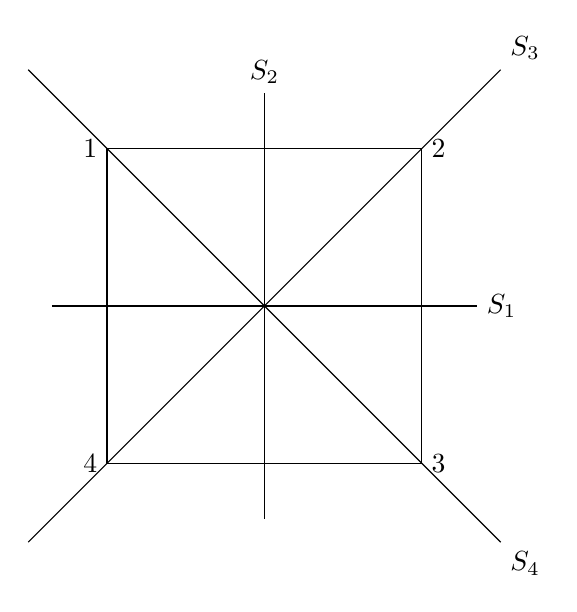
\begin{tikzpicture}
        \draw (0, 0) rectangle (4, 4) ;
        \node[left] at (0,0) {4};
        \node[right] at (4,0) {3};
        \node[right] at (4,4) {2};
        \node[left] at (0,4) {1};
        \draw (-0.7, 2) -- (4.7, 2) node[right] {$S_1$};
        \draw (2, -0.7) -- (2, 4.7)node[above] {$S_2$};
        \draw (-1, -1) -- (5, 5)node[above right] {$S_3$};
        \draw (-1, 5) -- (5, -1)node[below right] {$S_4$};
      \end{tikzpicture}
      \caption{正方形的对称群}
\end{figure}\label{fig:21}

\begin{exercise}
练习:证明整个群可以通过重复应用$R_{1}$和$S_{1}$来生成。
\end{exercise}
\begin{eg}
    一个$S_n$重要的子群是所有偶排列的集合,即$(-1)^{\pi}=1$,被称为交替群(alternating group),记作$A_n$。闭包性质,即两个偶排列的乘积总是偶排列,可以直接由式(2.1)得出。此外,标识排列id$_\mathrm{z}$显然是偶排列,而偶排列$\pi$的逆也必定是偶排列,因为
    \begin{equation}(-1)^{\pi\sigma}=(-1)^{\sigma\pi}=(-1)^{\pi}(-1)^{\sigma}.
    \end{equation}
   因此$A_n$是$S_n$的一个子群,阶数是$n!/2.$ 
\end{eg}
  
\begin{eg}
    设$\pi$是$1,2,\ldots,n$的任意排列,由于$n$个物体共有$n$!种排列,连续迭代$\pi^2,\pi^3,\ldots$最终会得到重复,即$\pi^k=\pi^l$,从而$\pi^{l-k}=\mathrm{id}_n$。满足$\pi^m=\mathrm{id}_n$的最小$m$被称为排列$\pi$的阶数(order of the permutation)。任何长度为$k$的周期显然有阶$k$,而由于任何排列都可以写成周期的乘积,排列的阶就是它的周期的最小公倍数。例如,(123)(45)的阶是3和2的最小公倍数,即6。元素$\{\mathrm{id}_n,\pi,\pi^2,\ldots,\pi^{m-1}=\pi^{-1}\}$形成$S_n$的子群,称为由$\pi$生成的子群。它显然是一个循环群。
\end{eg}
 
\section{矩阵群}
\subsection{线性变换}
$\mathbb{R}^{n}$是 $n\times 1$实列向量空间
\[\vec{x}=\begin{pmatrix}
    x_1\\x_2\\x_3\\\vdots\\x_n
\end{pmatrix}\]  
\subsection{矩阵群}
全体$n\times n$非奇异方阵组成一个群,记作 $GL(n,\mathbb{R})$ 原因在于行列式乘积法
\[\det(AB)=det(A)det(B)\] 
利用这一点可证明非奇异方阵可以组成一个群,满足封闭性,结合律以及可逆

在复数情况也可以做类似的讨论,记作$GL(n,\mathbb{C})$,与上面的实数情况并称为\textbf{n阶一般线性群}(general linear group of order n),其子群即群乘法为矩阵乘法的,统称为\textbf{矩阵群}(matrix groups)
\begin{eg}
    $n$阶的特殊线性群(special liner group)或称幺模群(unimodular group)记作$SL(n,\mathbb{R})$
\end{eg}
\section{同态和同构}
\subsection{同态}
两个群$G$和$G'$,映射$\varphi : G \rightarrow G'$保持群乘法,$$
\varphi(a b)=\varphi(a) \varphi(b)
$$
则称这个映射是同态 (homomorphism)
\begin{theorem}
    在同态映射下$G$的单位元映射到$G'$的单位元,任意元素之逆映为像元素之逆
\end{theorem}
\begin{proof}
    对于任意$g\in G$,
    $$
    \varphi(g)=\varphi(ge)=\varphi(g)\varphi(e).
    $$
    将上式两边同时乘以$(\varphi(g))^{-1}$可得到所需的结果。
    $$e'=e'\varphi(e)=\varphi(e)$$
    如果$g\in G$,则$\varphi(g^{-1})\varphi(g)=\varphi(g^{-1}g)=\varphi(e)=e^{\prime}$。因此$\varphi(g^{-1})=(\varphi(g))^{-1}$,满足要求。
     
\end{proof}
\begin{exercise}
    若 $\varphi: G\to G^{\prime}$ 是一个同态,证明像集
\begin{equation}\label{eq:2.13}
    \operatorname{im}(\varphi)=\varphi(G)=\{g'\in G'\mid g'=\varphi(g),\:g\in G\}        
\end{equation}
    是 $G^{\prime}$ 的子群。
\end{exercise}
\begin{eg}
    对任意实数$x\in \mathbb{R}$整数部分(integral part)记成$[x]$,小数部分(fractional part)写成$(x)=x-[x]$,显然$0 \leqslant(x)<1$\\
    在$[0,1]$区间上定义模\(1\)加法$$
    a+b \bmod 1=(a+b)
    $$
    这个群是阿贝尔的,称为实数模\(1\)群,\(a\)的逆元是\(1-a\),\(0\)的逆元是\(0\),\\
    映射$\varphi_{1}: \mathbb{R} \rightarrow [0,1]$,$\varphi_{1}(x)=(x)$保模\(1\)加法,即$((x)+(y))=(x+y)$\\
    类似的,$C(z)=\theta$,其中$z=|z| e^{i \theta}$,$0 \leqslant \theta<2 \pi$称为圆映射或相位映射\\
    是与复数的乘法群同态的,模$2\pi$加法群与上例类似
\end{eg}
\begin{eg}
    令$\operatorname{sign}:  S_{n} \rightarrow\{+1,-1\}$是分配给每个排列宇称的映射
    $$\operatorname{sign}(\pi)=(-1)^{\pi}=\begin{cases}
+1, & \text {若\(\pi\)为偶} \\
-1, & \text {若\(\pi\)为奇}
\end{cases}
$$
从\ref{sec:2.1}$\operatorname{sign}$是从到实数乘法群的同态$$
\operatorname{sign}(\pi \sigma)=\operatorname{sign}(\pi) \operatorname{sign}(\sigma)
$$
求行列式的映射$
\operatorname{det}: G L(n, \mathbb{R}) \rightarrow \dot{\mathbb{R}}
$也是一个同态
\end{eg}
\subsection{同构}
同构(isomorphism)是一一到上的同态映射,$G$和$G'$若存在同构映射,则称这两个群同构(isomorphic),记作$G \cong G^{\prime}$,这两个群在群性质上基本相同。

同构映射的逆映射和复合也都是同构的,这表明同构是一种等价关系,所以自然的我们有等价类,所以以后我们在指一个群时,往往指的是其等价类

群论是对同构群等价类的研究,通常,挑出一个等价的特殊代表是好事
\begin{theorem}[Cayley]
    任意$n$阶有限群都同构于排列群

    证明:对于每一个$g\in G$,定义映射$L_{g} : G\to G$为左乘以g,

    $$
    L_{g}(x)=gx\quad\mathrm{where}\quad x\in G.
    $$
    
    由于
    
    $$
    gx=gx^{\prime}\Longrightarrow x=x^{\prime}\quad\mathrm{and}\quad x=L_{g}(g^{-1}x)\quad\mathrm{for~all~}x\in G.
    $$
    
    因此,这个映射是一一对应和可逆的。$L_g$ 因此排列 $G=\{g_1=e,g_2,\ldots,g_n\}$ 的元素,并且可以被认为是$S_n$中的一个成员。它有属性 $L_g\circ L_h=L_{gh}$,因为
    
    $$
    L_{g}\circ L_{h}(x)=g(hx)=(gh)x=L_{gh}(x),\quad\forall x\in G.
    $$
    
    因此,由 $\varphi(g)=L_g$ 定义的映射 $\varphi:G\to S_n$ 是一个同态,
    
    $$
    \varphi(g)\varphi(h)=L_{g}\circ L_{h}=L_{gh}=\varphi(gh).
    $$
    
    此外,$\varphi$ 是一一对应的,因为如果 $\varphi(g)=\varphi(h)$ 那么 $g=L_g(e)=L_h(e)=h$ 。因此,$G$ 与 $\varphi(G)\subseteq S_{n}$ 的子群是同构的。
\end{theorem}
抽象上看两个群可能并没有什么不同,但同一群的不同“具体”版本可能有不同的应用,研究线性变换群或矩阵群的“具体”的理论称为群表示论。
\subsection{自同构和共轭类}
\textbf{自同构}(automorphism)指同构于自身的映射$\varphi: G \rightarrow G$

最平凡的例子:$\mathrm{id}_{G}: G \rightarrow G$(单位元)

自同构的复合还是自同构,逆亦然(封闭性)(逆元)

于是一个群的全体自同构映射也是一个群,记作$\operatorname{Aut}(G)$

对于任意的$g\in G$,映射$C_g:G\rightarrow G $定义成
\begin{equation}\label{eq:2.14}
    C_{g}(a)=g a g^{-1}
\end{equation}
成为由$g$导出的共轭(Conjugation),这个映射是同态的,因为$$
C_{g}(a b)=g a b g^{-1}=g a g^{-1} g b g^{-1}=C_{g}(a) C_{g}(b)
$$
$C_{g^{-1}}$是其逆,故$C_g$是$G$中的一个自同构,由$G$中的某些元素$g$导出的同构称为\textbf{内自同构}(inner automorphisms)

$C_{g h}=C_{g} \circ C_{h}$仍然成立,因为对任意$a\in G$
$$
C_{g} h(a)=g h a(g h)^{-1}=g h a h^{-1} g^{-1}=C_{g}\left(C_{h}(a)\right)
$$
所以映射 $\psi: G \rightarrow \operatorname{Aut}(G)$,定义成$\psi: G \rightarrow \operatorname{Aut}(G)$,也是同构的,这些内自同构,也就是 $\psi$  下 $G$  的像,组成一个 $\operatorname{Aut}(G)$的子群,两个子群\(H\)和\(H'\)通过 $G$的内自同构互相变换
$$
H^{\prime}=g H g^{-1}=\left\{g h g^{-1} \mid h \in H\right\}
$$
共轭也也在\(G\)上诱导出个等价关系:$a \equiv b$当且仅当存在\(g\in G\) 使 $b=C_{g}(a)$,(反身、对称和传递性都保持)遵循这种等价关系的等价类称为\textbf{共轭类}(conjugacy classes)

元素$a$的共轭类记作 $C_a$,包含恒等元的共轭类总是单子集\(\{e\}\),

\begin{exercise}
    阿贝尔群的共轭类什么?\marginpar[right]{单子集(译者注)}
\end{exercise}
\begin{eg}
    对于矩阵群,矩阵$A$和\(B\)如果依靠一个相似变换
    \[B=SAS^{-1}\]彼此联系,那么他们就在同一个共轭类中,两个相似的矩阵拥有相同的行列式,迹,和本征值
    \begin{enumerate}
        \item $$
        \operatorname{det} \mathbf{B}=\operatorname{det} \mathbf{S} \operatorname{det} \mathbf{A}(\operatorname{det} \mathbf{S})^{-1}=\operatorname{det} \mathbf{A}
        $$
        \item 由于\begin{equation}\label{eq:2.15}
            \operatorname{tr} (AB)=\operatorname{tr} (BA)
        \end{equation}
        所以$$
        \operatorname{tr} B=\operatorname{tr}\left(S A S^{-1}\right)=\operatorname{tr}\left(S^{-1} S A\right)=\operatorname{tr}(I A)=\operatorname{tr} A
        $$
        \item $$
        A\mathbf{v}=\lambda \mathbf{v} \Longrightarrow B(S \mathbf{v})=SAS^{-1} S \mathbf{v}=SA \mathbf{v}=\lambda S\mathbf{v}
        $$
    \end{enumerate}
\end{eg}
\begin{eg}
    易证,排列群\(S_3\)的共轭类是(用循环符号)
    \begin{enumerate}
        \item $\{e\}$
        \item $\{(12),(13),(23)\}$
        \item $\{(123),(132)\} $
    \end{enumerate}
    共轭类由具有相同循环结构的排列组成,是排列群的一个一般特征。
\end{eg}
\section{正规子群和商群}
\subsection{陪集}
对于一个群\(G\)的任意一对子集\(A\)和\(B\),定义\(AB\)是集合
$$A B=\{a b \mid a \in A,b \in B\}$$
如果\(H\)是\(G\)的子群那么\(HH=H\)

如果$H$是$G$的一个子群,那么$HH=H$。当$A$是一个单子集时,假设$A=\{a\}$,我们通常将$aB$写成 $\{a\}B$。如果$H$是$G$的一个子群,那么每个$a H$(其中$a \in G$)的子集称为$H$的\textbf{(左)陪集}(coset)。给定子群$H$的两个陪集要么相同,要么不相交。因为,假设存在元素$g \in aH \cap bH$

$$g=a h_{1}=b h_{2} \quad\left(h_{1}, h_{2} \in H\right)$$

对于任何$h \in H$,我们有

$$
a h=b h_{2} h_{1}^{-1} h \in b H \text {, }
$$

因此$a H \subseteq b H$。同样,可以证明$b H \subseteq a H$,因此$a H \cap b H=\emptyset$或$a H=b H$。由于$g=ge$且$e \in H$,所有$g \in G$都属于$gH$陪集。因此,$H$的陪集构成覆盖整个$G$的不相交子集族。还有另一种方法来证明这种分割属性。在$G$上定义的关系$a \equiv b$

$$
a \equiv b \quad \text { iff } \quad b^{-1} a \in H
$$

是一种等价关系,因为它是(i)反射,$a^{-1} a=e \in H$; (ii)对称,$a^{-1} b=$ $\left(b^{-1} a\right)^{-1} \in H$如果$b^{-1} a \in H$; 和(iii)传递,$a^{-1} b \in H, b^{-1} c \in H$ 诱导出 $a^{-1} c=a^{-1} b b^{-1} c \in H$。由此定义的等价类正是子群$H$的左陪集,因为$b \equiv a$当且仅当$b \in a H$。

\begin{theorem}[拉格朗日Lagrange]\label{thm:lagrange}
    如果$G$是一个有限群,那么每个子群$H$的阶数都是$n$的一个约数
\end{theorem}
    \begin{proof}
    每个余类$gH$与$H$之间存在一一对应关系,因为如果$gh_1=gh_2$,那么$h_1=g^{-1}gh_2=h_2$。因此,每个余类$gH$必须有完全相同的$|H|$个元素,由于余类划分了群$G$,因此$n$是$|H|$的倍数。
\end{proof}
    
    \begin{corollary}
        任意元素的阶是$|G|$的约数。
    \end{corollary}
    
    \begin{proof}
        设$g$是$G$的任意元素,$m$是它的阶。根据例2.5,$\left\{g, g^{2}, \ldots, g^{m}=e\right\}$这些元素彼此不相等,构成了阶数为$m$的循环子群。根据Lagrange定理,$m$整除群$G$的阶$|G|$。
    \end{proof}
    
    \begin{exercise}
        如果$G$的阶$p$是质数,所有的子群都是平凡的——它们要么是单位子群$\{e\}$,要么就是$G$本身
    \end{exercise}
\subsection{正规子群}
子群 $H$ 的右余集 $H g$ 与左余集的定义完全类似。虽然一般来说右余弦和左余弦之间没有明显的关系,但有一类重要的子群它们是重合的。如果符合以下条件,则称为群 $G$ 的正规子群(normal subgroup) $N$

$$
g N g^{-1}=N, \quad \forall g \in G
$$

这类子群是内自同构不变的;它们有时也被称为不变子群或自共轭子群。正规子群的关键特征在于左右陪集是相同的。
$$
g N=g N g^{-1} g=N g, \quad \forall g \in G
$$

这个论证可能会给人一种误解,即 $N$ 的每个元素都与 $G$ 的每个元素相乘,但它实际上证明了,对于 $N$ 中的每个 $n$ 和 $G$ 中的每个 $g$,都存在一个 $N$ 中的 $n^{\prime}$ 元素,使得 $g n=n^{\prime} g$。一般来说,我们没有理由认为$n^{\prime}=n$。

对于任何群$G$,平凡子群$\{e\}$和$G$总是正规的。如果一个群只有这些平凡子群以外没有其他正规子群
\begin{eg}
    群$G$的中心$Z$被定义为与$G$的所有元素都相互满足交换律的元素集合
    $$
Z=\{z \in G \mid z g=g z \text {对于全体 } g \in G\}
$$

这个集合构成了$G$的子群,因为三个基本要求都成立:

封闭性:如果$z, z^{\prime} \in Z$,那么$z z^{\prime} \in Z$,因为

$$
\left(z z^{\prime}\right) g=z\left(z^{\prime} g\right)=z\left(g z^{\prime}\right)=(z g) z^{\prime}=(g z) z^{\prime}=g\left(z z^{\prime}\right) \text {. }
$$

单位元:$e \in Z$,因为对于所有$g \in G$,$e g=g e=g$。

逆元:如果$z \in Z$,那么$z^{-1} \in Z$,因为

$$
z^{-1} g=z^{-1} g e=z^{-1} g z z^{-1}=z^{-1} z g z^{-1}=g z^{-1}
$$

由于对于所有$g \in G$,$g Z=Z g$,这个子群显是正规的
\end{eg}
\subsection{商群}
当我们将子群$H$的左陪集相乘时,例如
$$
g H g^{\prime} H=\left\{g h g^{\prime} h^{\prime} \mid h, h^{\prime} \in H\right\},
$$
一般来说,结果不是另一个陪集。另一方面,正规子群$N$的陪集的乘积总是另一个陪集,
$$
g N g^{\prime} N=g g^{\prime} N N=\left(g g^{\prime}\right) N,
$$
并且满足结合律,

$$
\left(g N g^{\prime} N\right) g^{\prime \prime} N=\left(g g^{\prime} g^{\prime \prime}\right) N=g N\left(g^{\prime} N g^{\prime \prime} N\right)
$$
此外,陪集$e N=N$扮演着一个单位元的角色,而每个陪集都有一个逆元 $(g N)^{-1}=g^{-1} N$。因此,正规子群$N$的陪集形成一个群,称为由$G$除以$N$的商群,表示为$G / N$。
\begin{eg}
    偶数整数$2 \mathbb{Z}$形成了整数和群$\mathbb{Z}$的正规子群,因为这是一个阿贝尔群。因子群$\mathbb{Z} / 2 \mathbb{Z}$只有两个陪集$[0]=0+2 \mathbb{Z}$和$[1]=1+2 \mathbb{Z}$,并且同取模2的加法群 $\mathbb{Z}_{2}$  同构(参见例2.4)。
\end{eg}

\subsection{同态的核}
设$\varphi: G \rightarrow G^{\prime}$是两个群$G$和$G^{\prime}$之间的同态,$\varphi$的核(kernel),用$\operatorname{ker}(\varphi)$表示,是$G$中那些映射到$G^{\prime}$中单位元$e^{\prime}$的元素的子集,

$$
\operatorname{ker}(\varphi)=\varphi^{-1}\left(e^{\prime}\right)=\left\{k \in G \mid \varphi(k)=e^{\prime}\right\}
$$

任何同态$\varphi$的核$K=\operatorname{ker}(\varphi)$都是$G$的子群:

封闭性:如果$k_{1}$和$k_{2}$属于$K$,那么$k_{1} k_{2}$也属于$K$,因为

$$
\varphi\left(k_{1} k_{2}\right)=\varphi\left(k_{1}\right) \varphi\left(k_{2}\right)=e^{\prime} e^{\prime}=e^{\prime} .
$$

单位元:$e \in K$,因为$\varphi(e)=e^{\prime}$

逆元:如果$k \in K$,那么$k^{-1} \in K$, for

$$
\varphi\left(k^{-1}\right)=(\varphi(k))^{-1}=\left(e^{\prime}\right)^{-1}=e^{\prime} .
$$

此外,由于对于所有$k \in K$和$g \in G$,$$\varphi\left(g k g^{-1}\right)=\varphi(g) \varphi(k) \varphi\left(g^{-1}\right)=\varphi(g) e^{\prime}(\varphi(g))^{-1}=e^{\prime}$$,因此K是一个正规子群。接下来的定理将证明这个结果的逆也成立,即每个正规子群都是某个同态的核。
\begin{theorem}
    设G为一个群。则以下两个性质成立:

\begin{enumerate}
  \item 如果$N$是$G$的一个正规子群,那么就有一个同态映射$\mu: G \rightarrow G / N$。

  \item 如果$\varphi: G \rightarrow G^{\prime}$是一个同态映射,那么因子群$G / \operatorname{ker}(\varphi)$和式(2.13)定义的像子群$\operatorname{im}(\varphi) \subseteq G^{\prime}$是同构的。

\end{enumerate}

$$
\operatorname{im}(\varphi) \cong G / \operatorname{ker}(\varphi)
$$
\end{theorem}
\begin{proof}
    \begin{enumerate}

\item 映射$\mu: G \rightarrow G / N$ 定义为 $\mu(g)=g N$ 是一个同构,因为
$$
\mu(g) \mu(h)=g N h N=g h N N=g h N=\mu(g h) \text {. }
$$

\item 设 $K=\operatorname{ker}(\varphi)$ 和 $H^{\prime}=\operatorname{im}(\varphi)$。在每个陪集$g K$上,映射$\varphi$都是常数,因为

$$
k \in K \quad \Longrightarrow \quad \varphi(g k)=\varphi(g) \varphi(k)=\varphi(g) e^{\prime}=\varphi(g)
$$

因此,我们只需要设

$$
\psi(g K)=\varphi(g)
$$

这种映射$\varphi$定义了映射$\psi: G / K \rightarrow H^{\prime}$,该映射是一个同构,因为

$$
\psi(g K h K)=\psi(g h K)=\varphi(g h)=\varphi(g) \varphi(h)=\psi(g K) \psi(h K)
$$

此外,$\psi$是一对一的,因为

$$
\begin{aligned}
\psi(g K)=\psi(h K) & \Longrightarrow \varphi(g)=\varphi(h) \\
& \Longrightarrow \varphi\left(g h^{-1}\right)=\varphi(g)(\varphi(h))^{-1}=e^{\prime} \\
& \Longrightarrow g h^{-1} \in K \\
& \Longrightarrow g \in h K .
\end{aligned}
$$

由于像集$H^{\prime}$中的每个元素$h^{\prime}$都是以$h^{\prime}=\varphi(g)=\psi(g K)$的形式出现的,因此映射$\psi$是群$G / K$和$H^{\prime}$之间的一个同构。
\end{enumerate}
\end{proof}
\begin{eg}
设$G$和$H$分别为两个具有恒等元$e_{G}$和$e_{H}$的群。可以在笛卡尔积$G \times H$上定义一个合成律,即

$$
(g, h)\left(g^{\prime}, h^{\prime}\right)=\left(g g^{\prime}, h h^{\prime}\right)
$$

这个乘积显然满足结合律,并且具有恒等元$\left(e_{G}, e_{H}\right)$。此外,每个元素都有唯一的逆元$(g, h)^{-1}=\left(g^{-1}, h^{-1}\right)$。因此,由于这个组合律,$G \times H$是一个称为$G$和$H$的直积的群。显然,群$G$与子群$\left(G, e_{H}\right)=\left\{\left(g, e_{H}\right) \mid g \in G\right\}$是同构的。后者是一个正规子群,因为

$$
(a, b)\left(G, e_{H}\right)\left(a^{-1}, b^{-1}\right)=\left(a G a^{-1}, b e_{H} b^{-1}\right)=\left(G, e_{H}\right)
$$

通常将元素$\left(G, e_{H}\right)$的子群与群$G$认为是相同的。类似地,$H$被认为与正规子群$\left(e_{G}, H\right)$等同。
\end{eg}
\section{群作用}\label{sec:2.6}
一个群$G$在集合$X$上的左作用是$G$到变换群$\operatorname{Transf}(X)$的同态:
$$
\varphi: G \rightarrow \operatorname{Transf}(X)
$$
通常将$\varphi(g)(x)$简写为$g x$,这样可以将$g h x$简写成$(g h) x$,因为
$$
(g h) x=\varphi(g h)(x)=\varphi(g) \varphi(h)(x)=\varphi(g)(h x)=g(h x) .
$$
群$G$在$\mathbb{R}^{n}$上的左作用$\phi$,其所有像都是线性变换,它是一个单射:
$$
\phi: G \rightarrow G L(n, \mathbb{R})
$$
它被称为wei$G$的\textbf{$n$维表示(n-dimensional representation)}。类似地,同态$\phi: G \rightarrow$ $G L(n, \mathbb{C})$被称为$G$的\textbf{复$n$维表示(complex n-dimensional representation)}。

\textbf{反同态(anti-homomorphism)}是定义为具有性质的映射$\rho: G \rightarrow \operatorname{Transf}(X)$:
$$
\rho(g h)=\rho(h) \rho(g)
$$
它可以产生右作用$x g=\rho(g)(x)$,这个表达式与写成$x g h$代替$x(g h)=(x g) h$是一致的。
\begin{exercise}
    如果$\varphi: G \rightarrow H$是一个同态,证明由$\rho(g)=\varphi\left(g^{-1}\right)$定义的映射$\rho: G \rightarrow H$是一个反同态。 

\end{exercise}
设G有一个左作用在X上,点x的\textbf{轨道}(orbit)$G x$是可以通过这个作用从x到达的所有点的集合: 
$$
G x=\{g x \mid g \in G\} \text {. }
$$ 

如果整个X都是某个点X的轨道,我们就说G对X的作用是\textbf{遍历的(transitive)}: 
$$
\exists x \in X \quad \text {使得} \quad X=G x
$$ 

在这种情况下,任何一对元素$y, z \in X$都可以通过群元素的作用连接起来,因为如果$y=g x$和$z=h x$,那么$z=g^{\prime} y$,其中$g^{\prime}=h g^{-1}$。因此,对于所有$y \in X$,$X=G y$。 

如果$x$是X的任意一点,定义x的\textbf{各向同性群(isotropy group)}为: 
$$
G_{x}=\{g\mid g x=x\}
$$ 

如果$g x=x \Longrightarrow g=\mathrm{id}_{X}$,那么G对X的作用就被称为自由的。 在这种情况下,各向同性群是平凡的,$G_{x}=\left\{\operatorname{id}_{X}\right\}$,对于每一点$x \in X$。 
\begin{exercise}
    证明$G_{x}$形成G的子群。
\end{exercise}

如果$x \in X$和$h, h^{\prime} \in G$,那么: 
$$
h x=h^{\prime} x \Longrightarrow h^{-1} h^{\prime} \in G_{x} \Longrightarrow h^{\prime} \in h G_{x}
$$ 

如果G是一个有限群,我们用$|S|$表示任何子集S中的点的数量。 由于$h G_{x}$是子群$G_{x}$的左陪集,而且根据Lagrange定理\ref{thm:lagrange}的证明,所有的陪集都有相同数量的元素,因此必须有正好$\left|G_{x}\right|$个群元素将x映射到其轨道$G x$的任何点$y$。 因此
\begin{equation} \label{eq:2.16}  
    |G|=|G x|\left|G_{x}\right| 
\end{equation}
\begin{eg}
2阶循环群$\mathbb{Z}_{2}=\{e, a\}$,其中$a^{2}=e$,对实数$\mathbb{R}$施加作用:
$$
e x=x, \quad a x=-x
$$

任意一点$x \neq 0$的陪集为$\mathbb{Z}_{2} x=\{x,-x\}$,而$\mathbb{Z}_{2} 0=\{0\}$。这一作用不是遍历的。原点的各向同性群是整个$\mathbb{Z}_{2}$,而其它任何点的各向同性群都是$\{e\}$。分别对于$x=0$和$x \neq 0$的情形分别检验 (2.16) 很简单。
\end{eg}
\begin{eg}
    实数加法群$\mathbb{R}$ 对复平面$\mathbb{C}$施行作用:
$$
\theta: z \mapsto z e^{i \theta}
$$
任意$z \neq 0$的轨道是围绕0为圆心、半径为$r=|z|$的圆。该作用不是遍历的,因为不同半径的圆是互不相交的。任意$z \neq 0$的各向同性群是形如$\theta=2 \pi n$ 的实数,其中$n \in \mathbb{Z}$。因此,对于$z \neq 0$的各向同性群$\mathbb{R}_{z}$与加法群$\mathbb{Z}$同构。另一方面,$z=0$的各向同性群是$\mathbb{R}$的全部元素。
\end{eg}
\begin{eg}
 一个群$G$通过左乘变换来作用于自身:
$$
g: h \mapsto L_{g} h=g h
$$
由于任何元素$g^{\prime}$都可以通过左乘变换从另一个$g$到达,因此这种作用显然是遍历的:
$$
g^{\prime}=L_{g^{\prime} g^{-1}} g
$$
任何子群$H \subseteq G$也会通过左乘变换来作用于$G$。在这种作用下,任何群元素$g$的轨道是包含$g$的右陪集$H g$。类似地,在$H$对$G$定义的右乘变换$R_{h}: g \mapsto g h$的作用下,轨道是左陪集$g H$。一般情况下,这些作用并不遍历。
\end{eg}
\begin{eg}
由元素$g$所定义的共轭过程,如式(\ref{eq:2.14})所示,是群$G$对其自身的左作用,因为映射$g \mapsto C_{g}$是一个同态,

$$
C_{g h} a=(g h) a(g h)^{-1}=g h a h^{-1} g^{-1}=C_{g} C_{h} a
$$

其中我们写$C_{g} a$ 代表$C_{g}(a)$。共轭作用的轨道正是共轭类。由式(\ref{eq:2.16})可知,如果$G$是一个有限群,那么任何共轭类中的元素数量,作为$G$作用的轨道,是群$|G|$的阶数的因数。

如果$G$在集$X$上有一个左作用,并且$x$和$y$是$X$中处于同一轨道的任意一对点,即$y=h x$,其中$h \in G$,那么它们的各向同性群是彼此共轭的,


\begin{equation}
    G_{y}=G_{h x}=h G_{x} h^{-1}
\end{equation}

因为,设$g \in G_{y}$,即$g y=y$。由于$y=h x$,因此应用$h^{-1}$得到$h^{-1} g h x=x$。因此$h^{-1} g h \in G_{x}$,或者等价地$g \in h G_{x} h^{-1}$。反之,即$h G_{x} h^{-1} \subseteq G_{y}$,是直接的:对于任何$g \in h G_{x} h^{-1}$,我们有

$$
g y=g h x=h g^{\prime} h^{-1} h x \quad \text { 其中 } \quad g^{\prime} \in G_{x},
$$

因此$g y=h x=y$和$g \in G_{y}$。因此,$x$和$y$的各向同性群是同构的,因为它们是彼此共轭的,并且是由内部自同构关联的。如果$G$对$X$的作用是遍历的,那么任意一对点$x$和$y$的各向同性群是彼此同构的。
\end{eg}
\begin{exercise}
    在什么情况下,元素 $g$ 对群 $G$ 的共轭作用是遍历的?
\end{exercise}

\section{对称群}
对于物理学家来说,对群的真正兴趣在于它们与相关空间或某些重要函数(如拉格朗日)的对称性之间的联系。在此,空间 $X$ 的概念将从最广义的角度来理解,指的是具有 "结构 "的集合 $X$,如第 1.6 节所述。这类空间的定义可能涉及代数和几何结构的组合,但关键是它们的定义总是涉及空间上某些函数的指定。例如,代数结构(如群)需要组成法则,即定义在底层集合的笛卡尔积上的函数。几何结构(如拓扑学)通常涉及对$X$子集的选择--这也可以定义为对$X$幂集的特征函数。就目前而言,让我们简单地把空间看作是一个集合 $X$ 连同一个或多个函数 $F: X \rightarrow Y$ 到定义在其上的另一个集合 $Y$。这个概念足够概括 "空间 "的基本概念。

如果$F$是$X$上的$Y$值函数,我们说变换$g: X \rightarrow X$保持$F$不变,如果

$$
F(x)=F(g x) \quad \text { for all } x \in X
$$

其中,正如第\ref{sec:2.6}节中所述,我们用$g x \equiv g(x)$表示左作用。
\begin{theorem}
    对于$X$上的所有使$F$不变的变换组成一个群。
\end{theorem}
\begin{proof}
    老三样:

封闭性:如果$g$和$h$使$F$不变,则对于所有$x \in X$,$F(x)=F(h x)$,对于所有$y \in X$,$F(y)=F(g y)$。因此$g h \equiv g \circ h$也使$F$不变,因为$F(g h x)=F(g(h x))=F(h x)=$ $F(x)$。

恒等元:很明显,$F(x)=F\left(\operatorname{id}_{X}(x)\right)$; 也就是说,$\mathrm{id}_{X}$使$F$不变。

逆元:如果$g$是一个变换,那么存在一个逆变换$g^{-1}$,使$g g^{-1}=\mathrm{id}_{X}$。如果$g$使$F$不变,那么$g^{-1}$也使$F$不变,因为

$$
F\left(g^{-1} x\right)=F\left(g\left(g^{-1} x\right)\right)=F(x) .
$$
\end{proof}
将上述定理推广到任意集合$\mathcal{F}$上的函数是一件很简单的事情。保持所有函数$F \in \mathcal{F}$不变的变换群将被称为$\mathcal{F}$的不变群或对称群。以下是数学物理学中一些重要的对称群例子。
\begin{eg}
    旋转群$SO(3)$。正如例2.11中所述,让$\mathbb{R}^3$是所有$3 \times 1$列向量的集合

$$
\mathbf{r}=\left(\begin{array}{l}
x \\
y \\
z
\end{array}\right) \quad  x, y, z \in \mathbb{R}
$$

考虑$\mathbb{R}^3$上所有线性变换$\mathbf{r} \mapsto \mathbf{r}^{\prime}=\mathrm{A} \mathbf{r}$,其中$\mathrm{A}$是一个$3 \times 3$矩阵,它将点到原点的距离$r=|\mathbf{r}|=\sqrt{x^{2}+y^{2}+z^{2}}$保持不变。由于$r^2=\mathbf{r}^T \mathbf{r}$,我们有

$$
r^{\prime 2}=\mathbf{r}^{\prime T} \mathbf{r}^{\prime}=\mathbf{r}^{T} \mathrm{~A}^{T} \mathrm{~A} \mathbf{r}=r^{2}=\mathbf{r}^{T} \mathbf{r}
$$

这对于任意矢量$\mathbf{r}$都成立,当且仅当$\mathrm{A}$是正交矩阵,$\mathrm{AA}^{T}=\mathrm{I}$。正如例2.11中所示,正交变换的行列式都为$\pm 1$ 。其中行列式为$+1$的叫做旋转,而行列式为$-1$的必须涉及一个平面上的反射;例如,变换$x^{\prime}=x, y^{\prime}=$ $y, z^{\prime}=-z$。
同样地,$O(n)$是$n$维距离函数的对称群,

$$
r=\sqrt{x_{1}^{2}+x_{2}^{2}+\cdots+x_{n}^{2}}
$$

其中行列式为正的则用$S O(n)$表示,称为$n$维空间的旋转群。我们假定这个群的变换都是线性变换,不会有任何损失,因为可以证明,任何使$r^{2}$保持不变的$\mathbb{R}^{n}$变换必须是线性的(参见第18章)。
\end{eg}

\begin{eg}
    欧氏群。欧氏空间 $\mathbb{E}^{3}$ 定义为笛卡尔空间$\mathbb{R}^{3}$,任意一对点之间的距离函数为:

$$
\Delta s^{2}=\left(\mathbf{r}_{2}-\mathbf{r}_{1}\right)^{2}=\Delta \mathbf{r}^{T} \Delta \mathbf{r}
$$
\end{eg}
